% cd ..\..\Users\NikitaSkybytskyi\Desktop\c3s2\ecology-and-economics\lab-3\tex
% cls && pdflatex -shell-escape report.tex && cls && pdflatex -shell-escape report.tex && del report.aux, report.toc, report.log, report.out && start report.pdf
\documentclass[12pt, a4paper]{article}
\usepackage[T2A]{fontenc}
\usepackage[utf8]{inputenc}
\usepackage[english,ukrainian]{babel}
\usepackage{amsmath, amssymb}

\usepackage[top = 2 cm, left = 1 cm, right = 1 cm, bottom = 2 cm]{geometry}

\usepackage{float, graphicx}

\usepackage{minted}

\newcommand*\diff{\mathop{}\!\mathrm{d}}

\setlength\parindent{0pt}
\allowdisplaybreaks

\newcommand{\cover}[2]{
\begin{center}
\hfill \break
	Міністерство освіти та науки України \\
	Київський національний університет імені Тараса Шевченка \\ 
	Факультет комп'ютерних наук та кібернетики \\
	Кафедра обчислювальної математики
\end{center}

\vfill 

\begin{center}
	\large{
		Звіт до лабораторної роботи №{#1} на тему: \\ 
		``{#2}'
	}
\end{center}

\vfill 

\begin{flushright}
	Виконав студент групи ОМ-3 \\
	Гронь Ілля
\end{flushright}

\vfill 

\begin{center}
    Київ, 2018 
\end{center}

\thispagestyle{empty} 
\newpage
}

\begin{document}

\cover{3}{Попит та пропозиція. Ринкова рівновага. \\ Стабільність рівноваги. Вплив дотації}

\tableofcontents

\section{Теоретичні відомості}



\section{Чисельне моделювання}

Було використано мову програмування \texttt{Python} і модуль \texttt{scipy}.

\subsection{Код}

\inputminted{python}{lab-3/py/all.py}
% \inputminted{python}{../py/all.py}

\subsection{Графіки}

\begin{figure}{H}
	\centering
	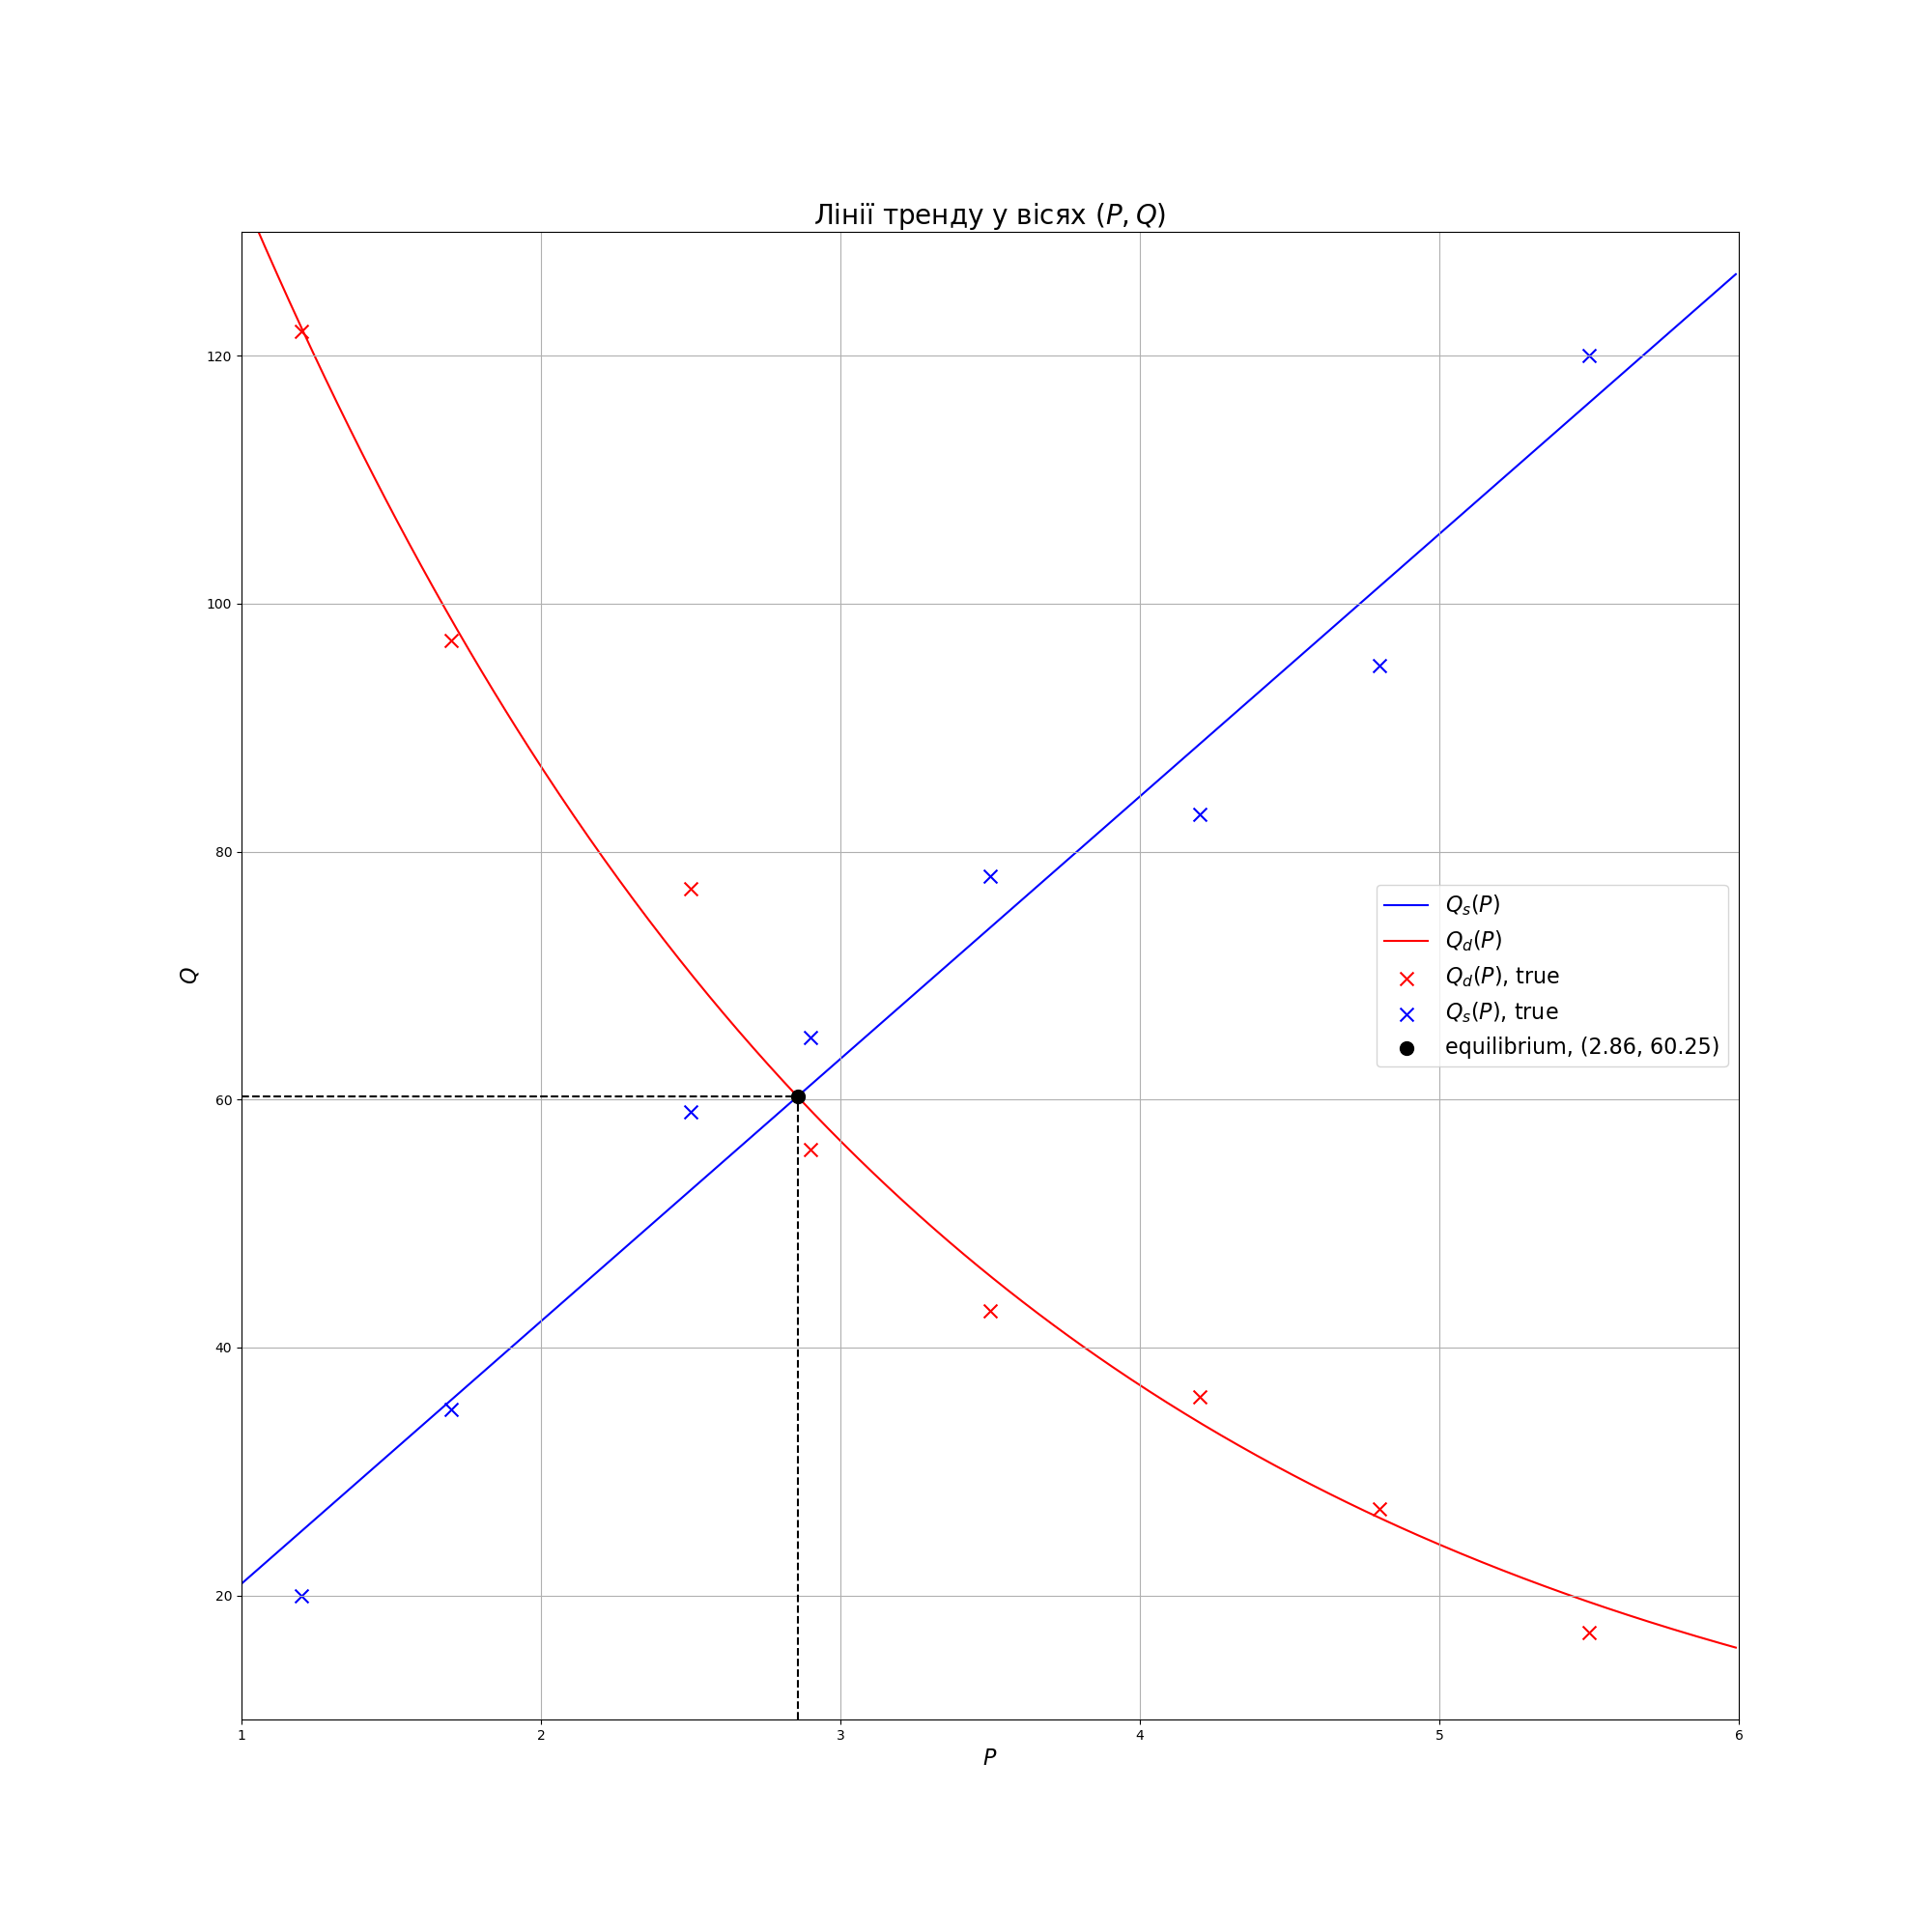
\includegraphics[width=\textwidth]{p_q.png}
\end{figure}

\begin{figure}{H}
	\centering
	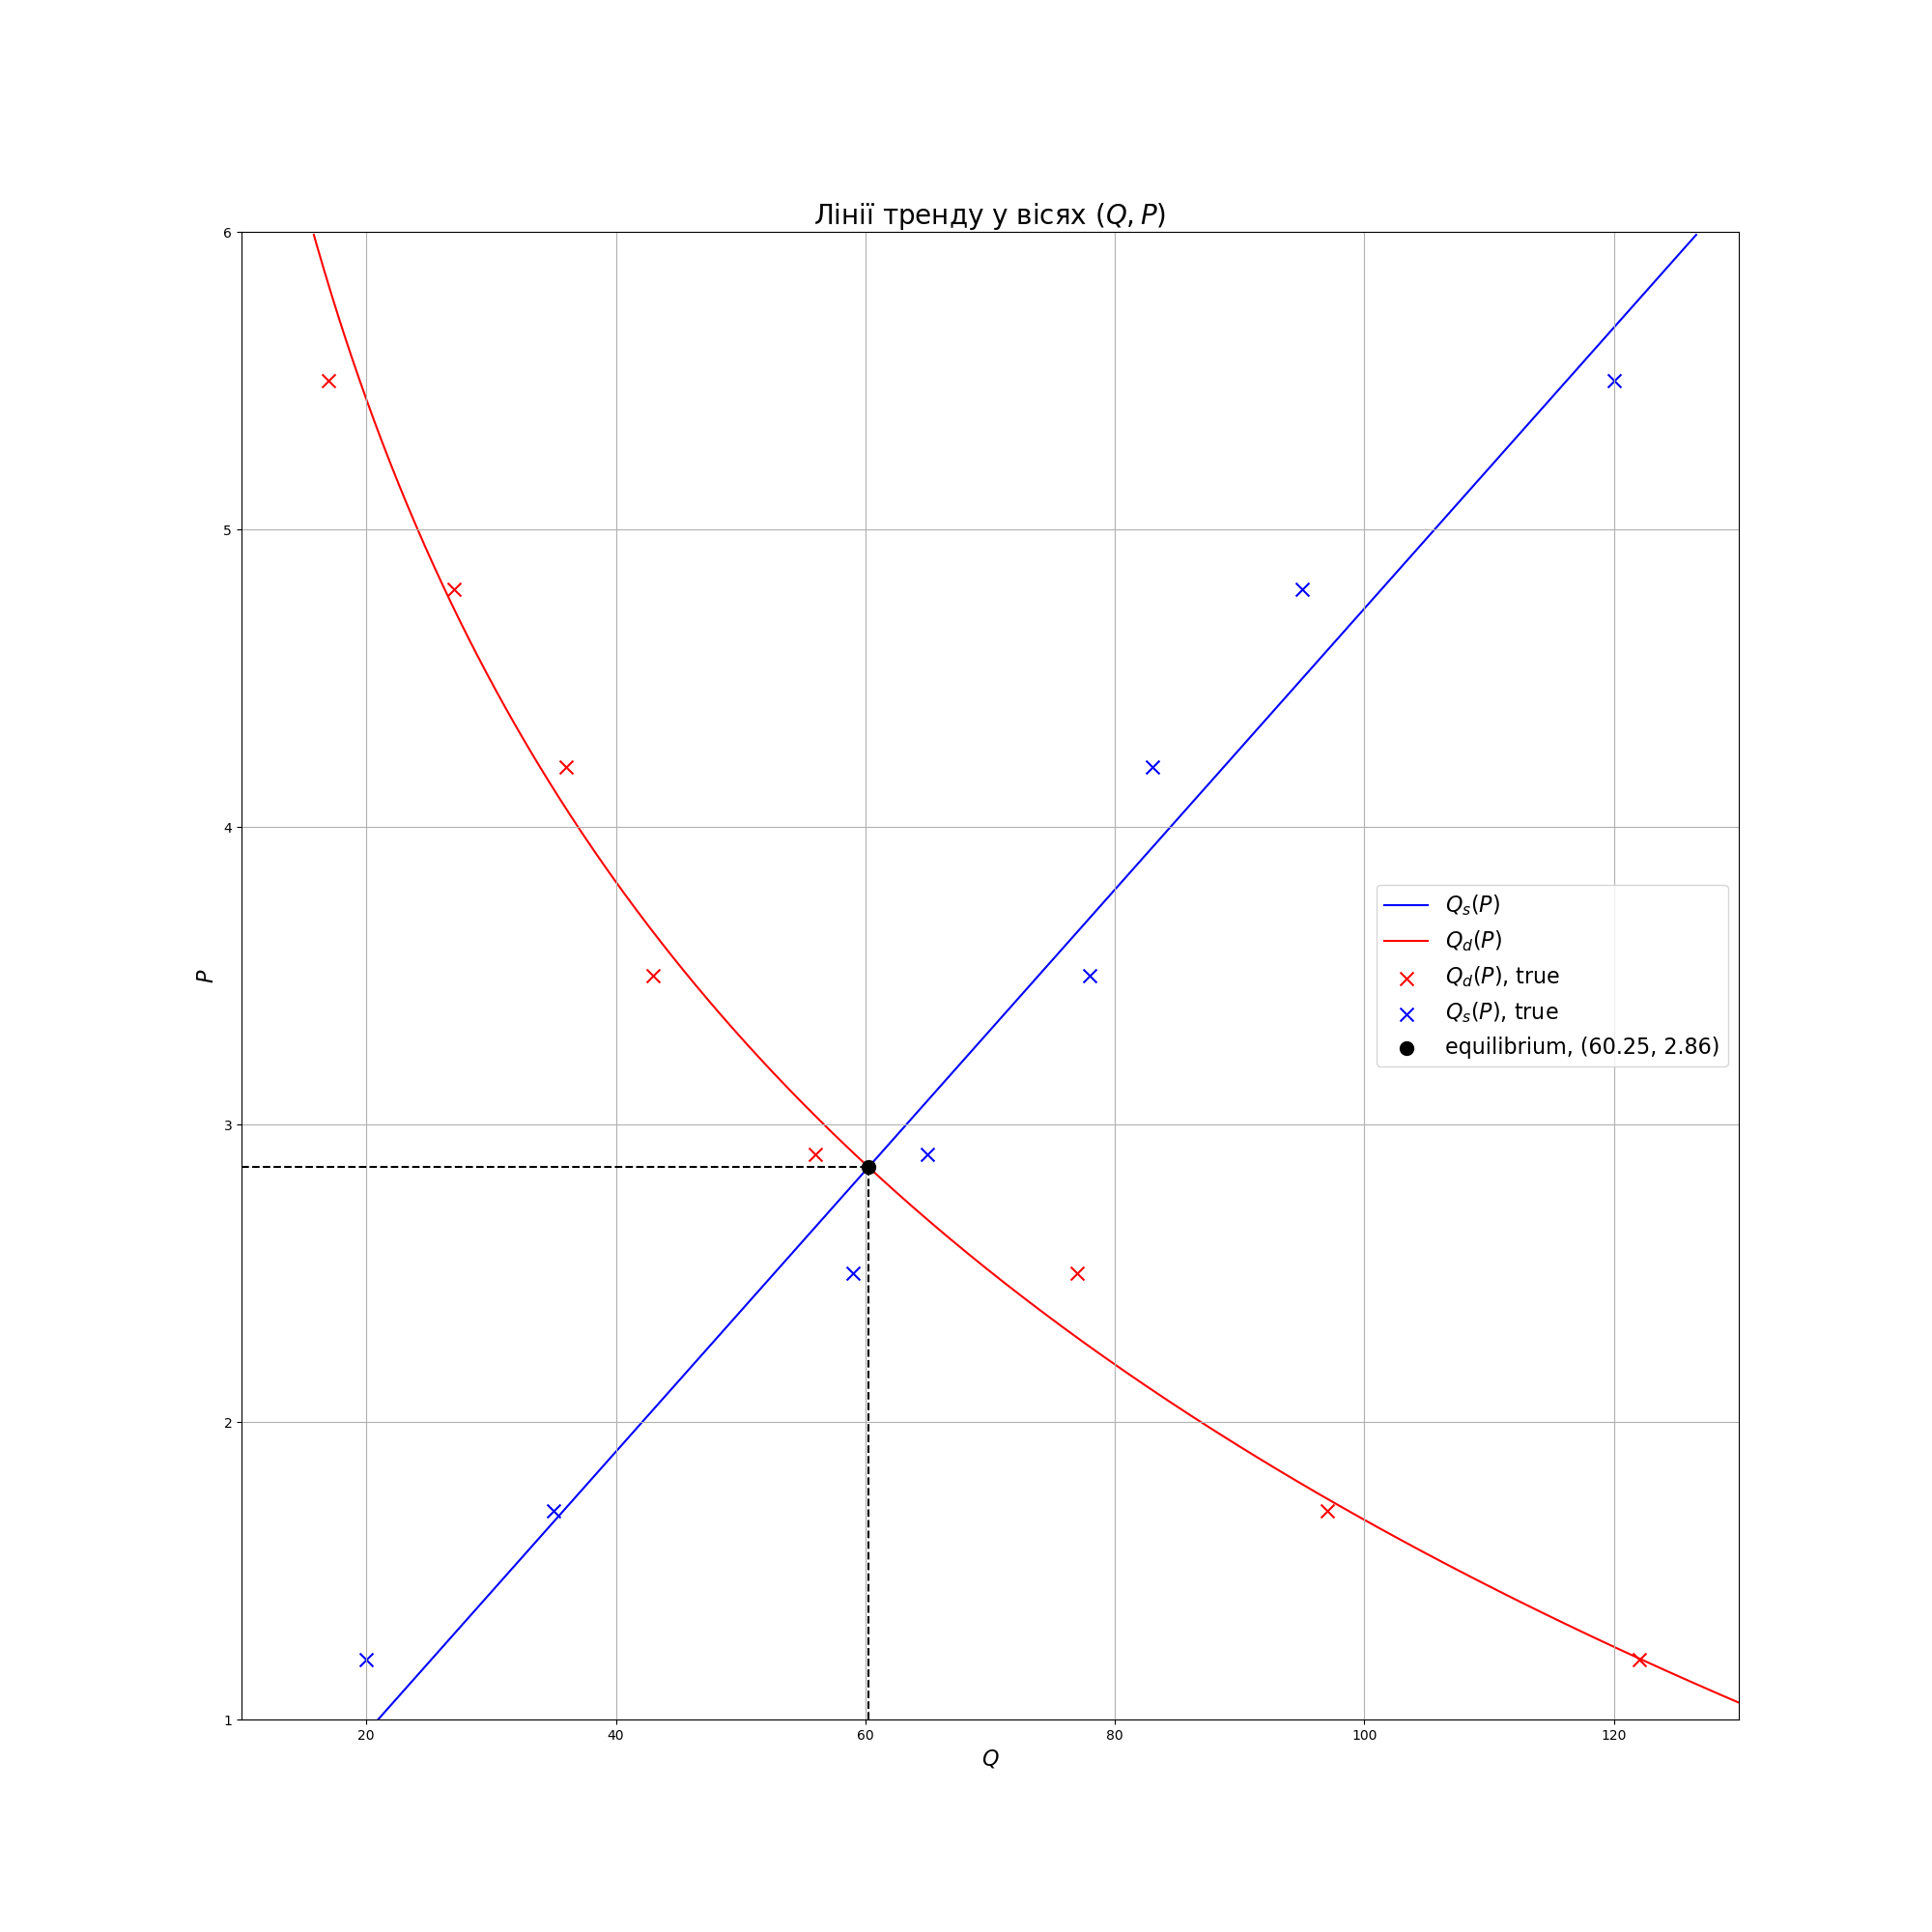
\includegraphics[width=\textwidth]{q_p.png}
\end{figure}

\begin{figure}{H}
	\centering
	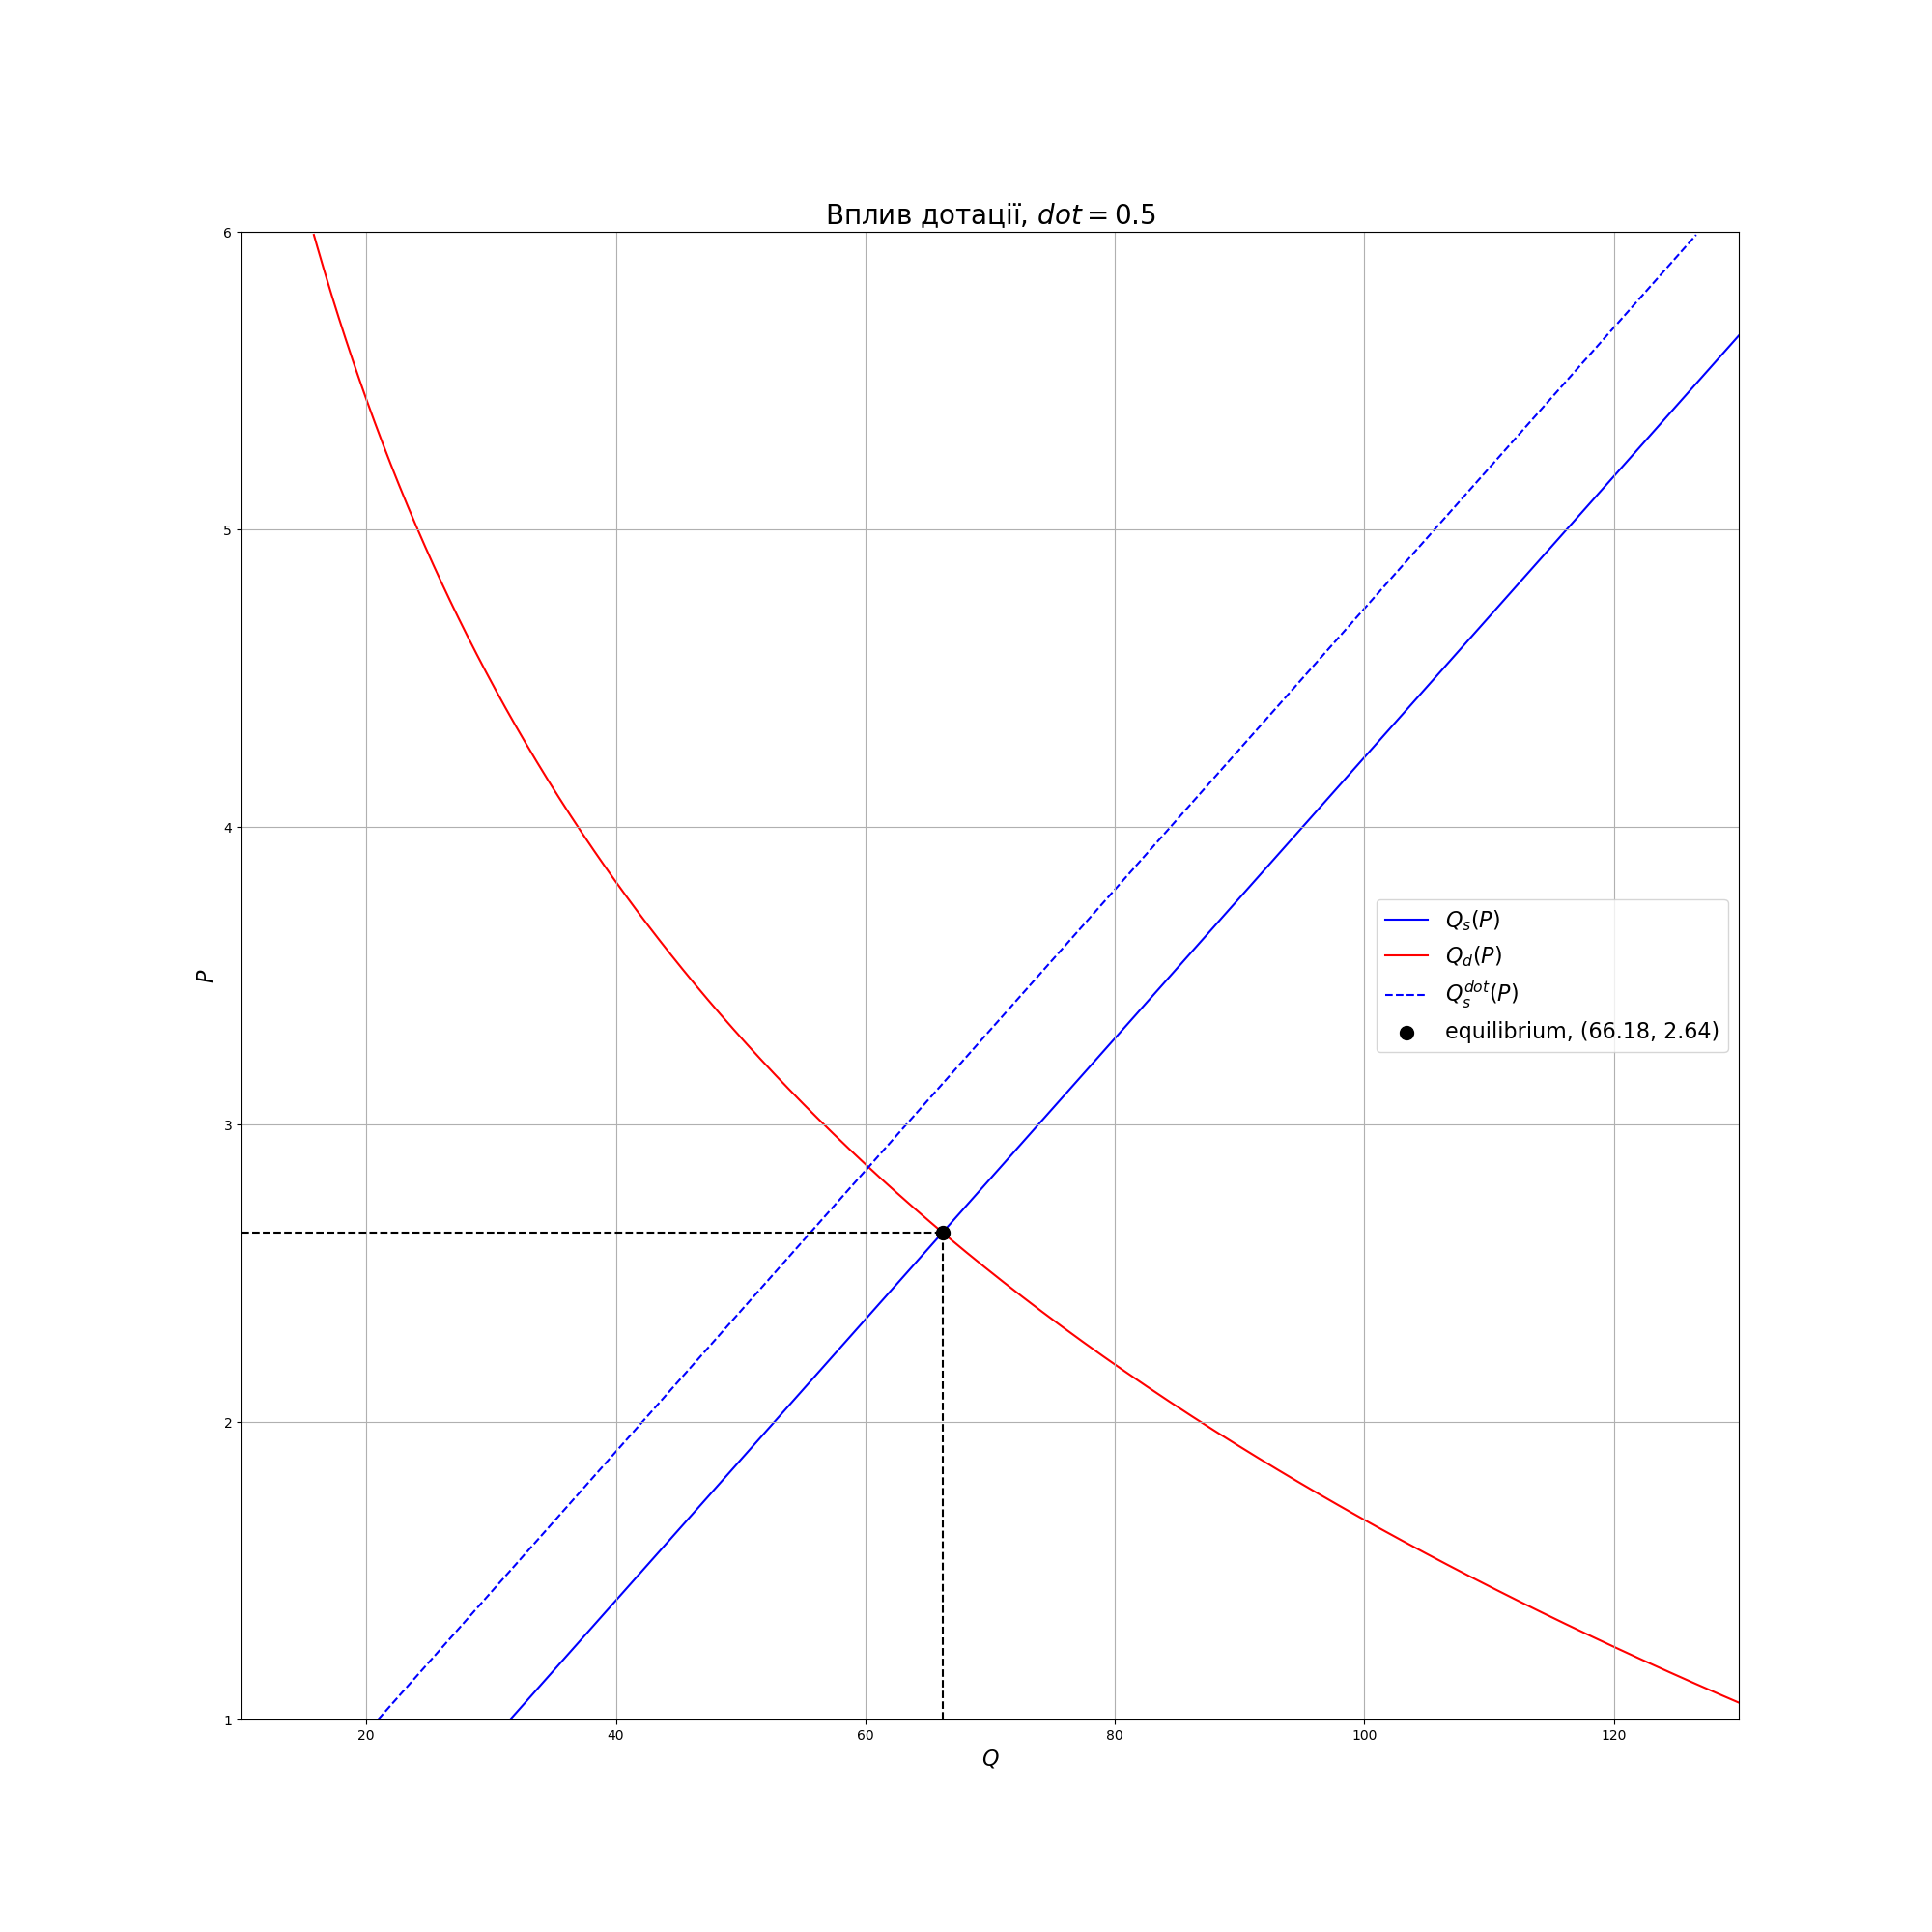
\includegraphics[width=\textwidth]{dotation.png}
\end{figure}

Як бачимо, отримані результати відповідають теоретичним очікуванням.

\end{document}